\chapter{Phase Transitions and Critical Phenomena}
\label{ch2-crit}

%sources
    %Henkel - Conformal Invariance and Critical Phenomena - Ch1
    %Gitterman - Ch1
    %Nishimore - Ch1
    %Sole - Ch1

    %DIFFUSION-LIMITED GROWTH IN BACTERIAL COLONY FORMATION Mitsugu MATSUSHITA a
    %and Hiroshi FUJIKAWA b (LDA FIG)
    %http://people.umass.edu/machta/images/dla.html

Lorem ipsum dolor sit amet, consectetur adipisicing elit, sed do eiusmod tempor
incididunt ut labore et dolore magna aliqua. Ut enim ad minim veniam, quis
nostrud exercitation ullamco laboris nisi ut aliquip ex ea commodo consequat.
Duis aute irure dolor in reprehenderit in voluptate velit esse cillum dolore eu
fugiat nulla pariatur. Excepteur sint occaecat cupidatat non proident, sunt in
culpa qui officia deserunt mollit anim id est laborum.


\begin{figure}
\begin{center}
    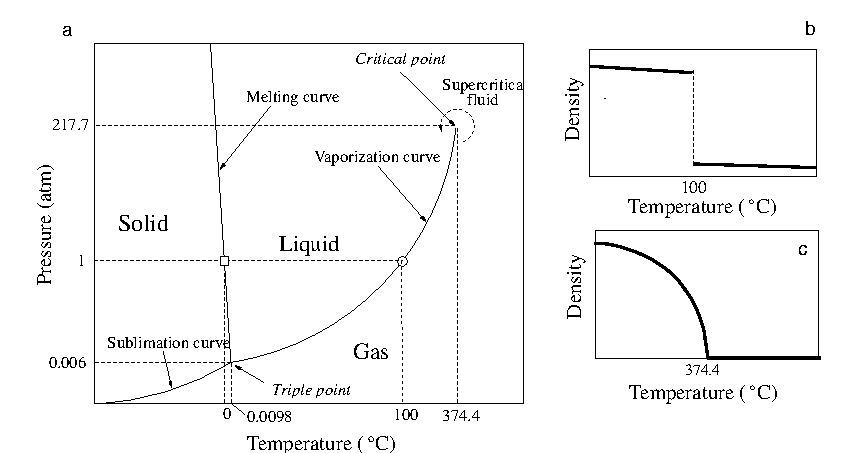
\includegraphics[scale=1.0]{chapters/ch2-crit/figs/water}
\end{center}
\caption{Phase diagram of water (a). Here, the three usual phases are
    distinguished, each separated from the other by a critical line. The
    phase transition that happens when the system traverse a line is
    characterized by a discontinuous jump in the density, as shown in (b) for
    the liquid-gas transition at $P=1$ atm. For $P=217.7$ atm however the same
    transition is continuous, as shown in (c). In the vicinity of this phase
    transition, at $T\approx374.4^\circ$C, the two phases become
    indistinguishable, and display a number of peculiarities. Such systems are
    called critical systems. Reproduced from [???].}
% taken from Sole - page 7
\label{fig:bacteria}
\end{figure}

\begin{figure}
\begin{center}
    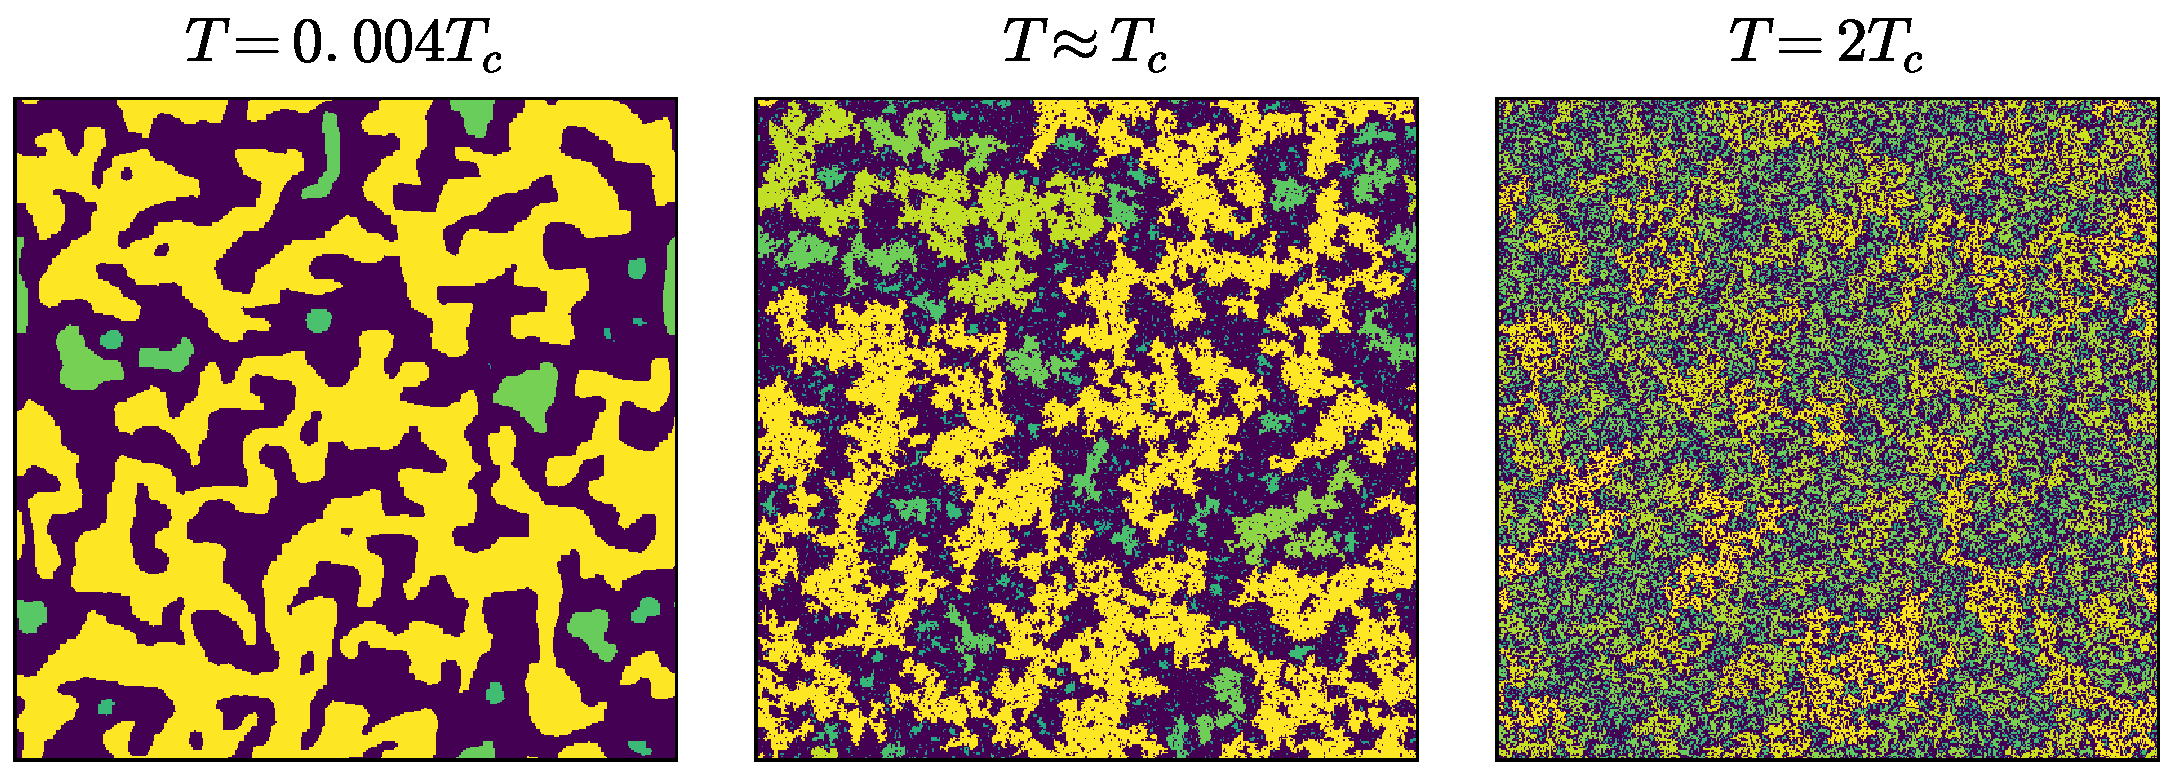
\includegraphics[scale=0.6]{chapters/ch2-crit/figs/ising}
\end{center}
\caption{Examples of three realizations of the Ising model with three different
    temperatures. The clusters of adjacent spin-up sites are colored according
    to how many sites belong to it. The subcritical regime is dominated by the
    large clusters. On the other side, above the critical point, the system is
    dominated by thermal fluctuations, undermining cluster formation. At the
    critical point however, the clusters lack a characteristic length scale.
    One can observe that the image has a certain ``depth'' to it. This happens
    because clusters of all sizes are present, a mark of scale invariance,
    the most important property of critical systems.}
\label{fig:bacteria}
\end{figure}

%\begin{figure}
%\begin{center}
    %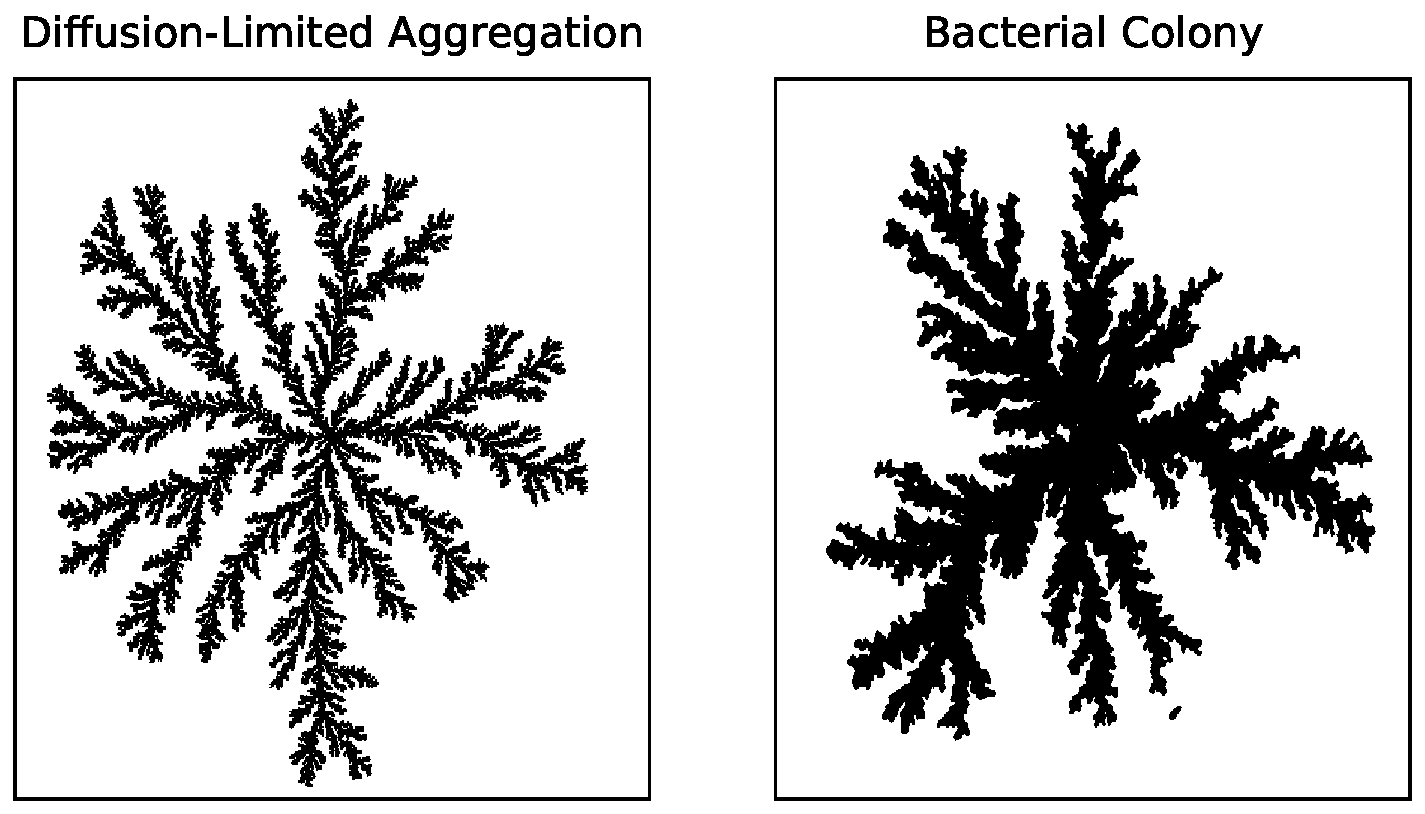
\includegraphics[scale=0.6]{chapters/ch2-crit/figs/bacteria}
%\end{center}
%\caption{Images taken from [???] and [???].}
%\label{fig:bacteria}
%\end{figure}
